\chapter{Implementation of the game}\label{ch:implementation}
\section{The Smart Contract}
	\begin{figure}[ht]
		\begin{center}
			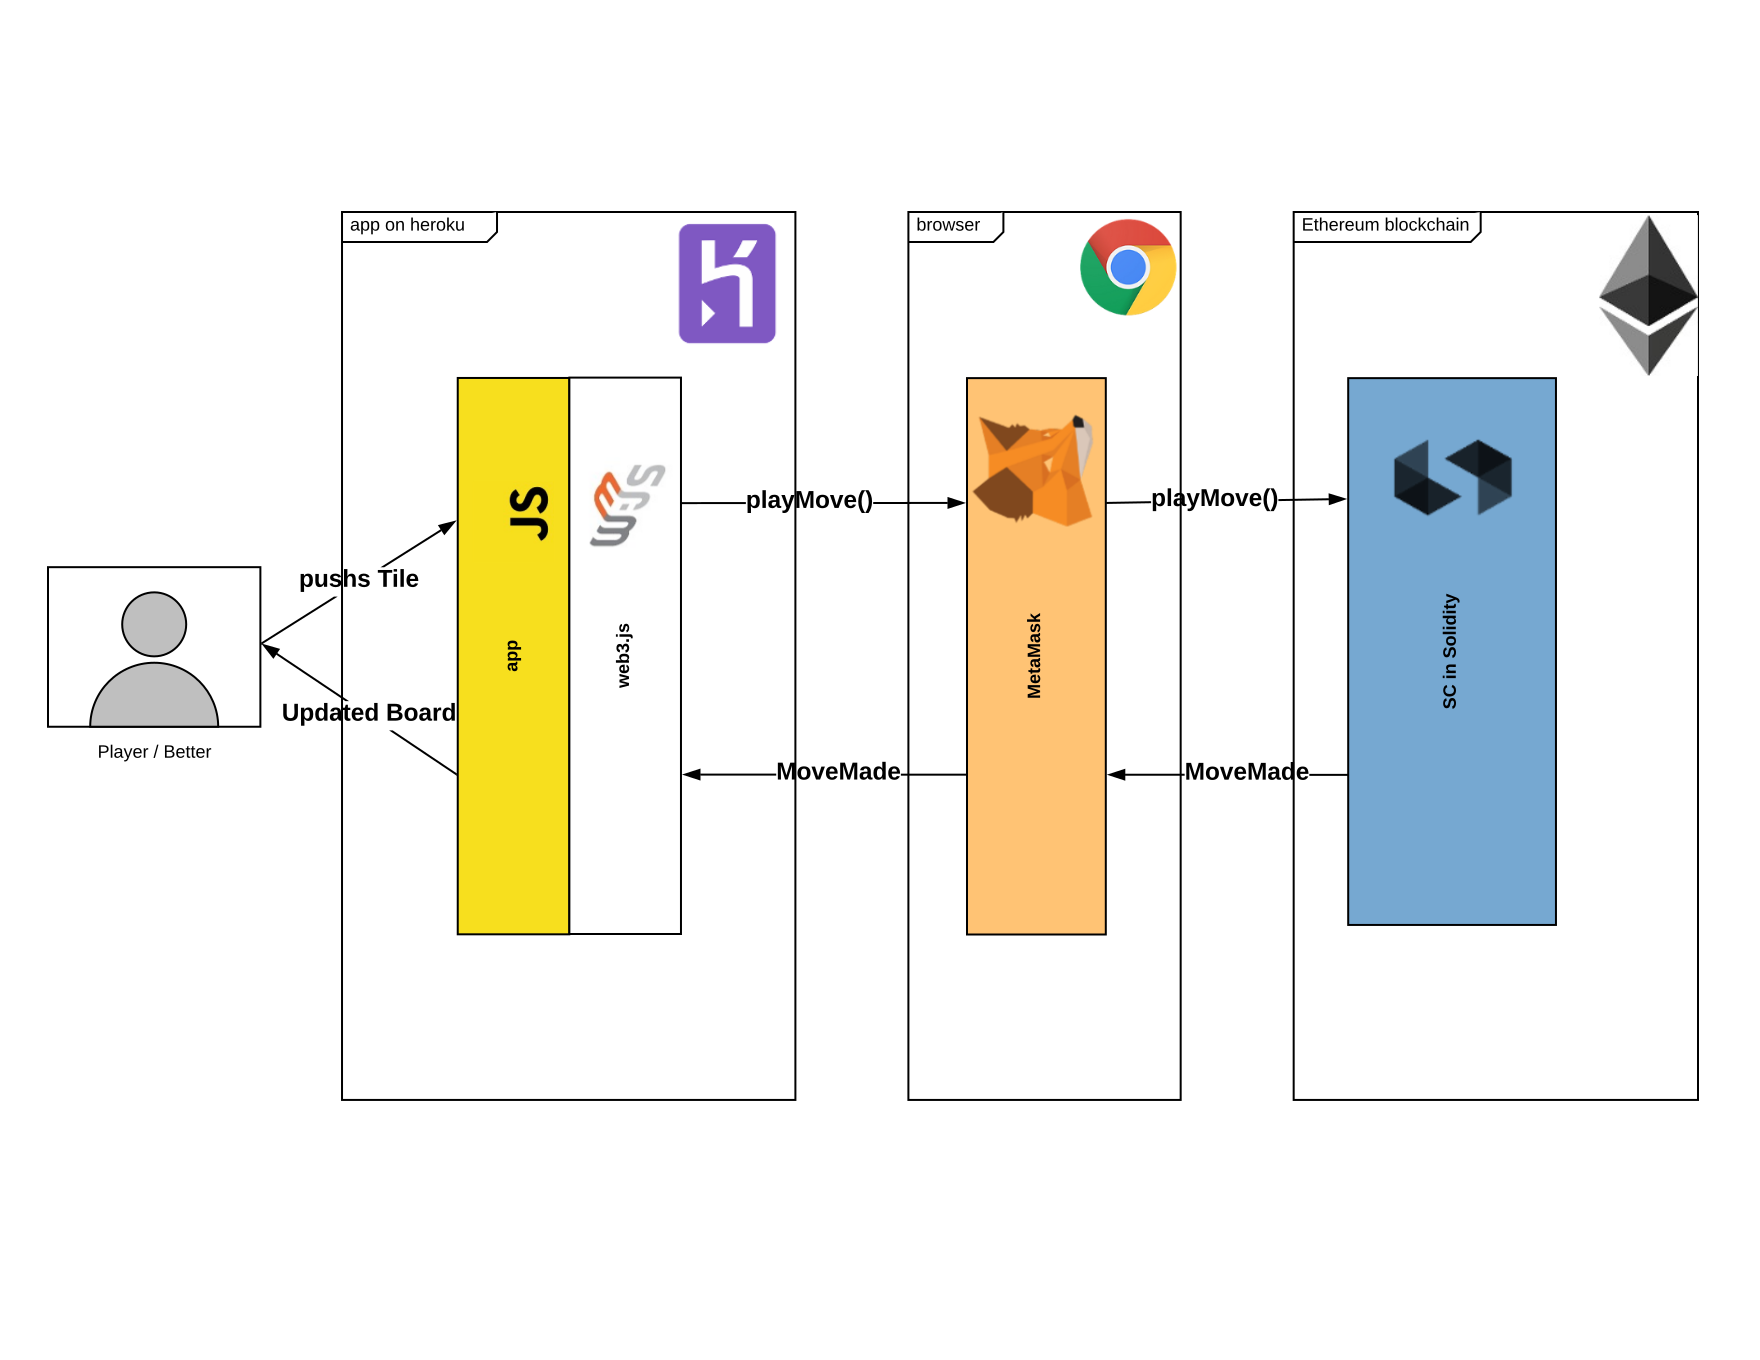
\includegraphics[scale=0.4]{res/project_structure}
		\end{center}
		\caption{Project Structure with Technologies}
		\label{fig:project_structure}
	\end{figure}	
Figure \ref{fig:project_structure} shows the project structure and the interaction between the different systems by the example of an Player choosing a tile on the board.
The web-application is running on the Heroku Platform\footnote{https://www.heroku.com/}. Through the browser and MetaMask a User can get verified by its Ethereum-account and pay the requested amount of gas in order to run functionalities on the Ethereum \ac{sc}. The \ac{sc} itself runs on an blockchain, which can be either a private or the Ropsten Testnet\footnote{https://ropsten.etherscan.io/}.\\
The \ac{sc} firstly checks if the move is valid. Secondly it looks for a winner and changes the game state if so. After that it returns a move confirmation to the user.

Three functions of the \ac{sc} we show here, as we consider them complex and interesting:\\


\subsection{1.Play Move Function\\}
	\begin{lstlisting}[language=JavaScript,escapechar=|]
event MoveMade(bool success, uint gameId, GameState state, uint x, uint y, string symbol);|\label{line:event}| 
function playMove(uint gameId, uint x, uint y) public { |\label{line:param}| 
	Game storage game = games[gameId];|\label{line:mapping}|
		    
	require(game.state >= GameState.X_HAS_TURN, "The game is not started yet.");
	require(game.state < GameState.WINNER_X, "The game is already finished.");
		    
	game.moveCounter += 1;
		    
	if (game.state == GameState.X_HAS_TURN) {
		require(game.playerXAddr == msg.sender
			|| game.moveCounter == boardSize * boardSize// last move made 	automatically
			, "Sender not equal player X");
		require(game.board[y][x] == SquareState.EMPTY
		,"Move not possible because the square is not empty.");
		    
		game.board[y][x] = SquareState.X;|\label{line:boardX}|
		game.state = GameState.O_HAS_TURN;
		checkForWinner(x, y, gameId, game.playerXAddr);|\label{line:winnerX}|
		    
		emit MoveMade(true, gameId, game.state, x, y, "X");|\label{line:emit1}|
	}
	else {
		require(game.playerOAddr == msg.sender
			|| game.moveCounter == boardSize * boardSize      // last move made automatically
			, "Sender not equal player O");
		require(game.board[y][x] == SquareState.EMPTY
			, "Move not possible because the square is not empty.");
		    
		game.board[y][x] = SquareState.O;|\label{line:boardO}|
		game.state = GameState.X_HAS_TURN;
		checkForWinner(x, y, gameId, game.playerOAddr);|\label{line:winnerO}|
		    
		emit MoveMade(true, gameId, game.state, x, y, "O");|\label{line:emit2}|
	}
	if (game.moveCounter == boardSize*boardSize - 1 && game.state < GameState.WINNER_X) {
		doLastMoveAutomatically(game);|\label{line:lastMove}|
	}
}
\end{lstlisting}

This functions gets called when a player clicks on a tile in order to make his move.The game id is send as an parameter (line \ref{line:param}). With this id the corresponding game object can be called through a mapping (line \ref{line:mapping})  It adds the players symbol into the specific location within the game-board firstly (line \ref{line:boardX} and \ref{line:boardO}). Afterwards it calls the 'checkForWinner' function (line \ref{line:winnerX} and \ref{line:winnerO}). The event MoveMade (line \ref{line:event}) is triggered returning the user an confirmation of the move (line \ref{line:emit1} and \ref{line:emit2}). There is also an an auto completion for the last move if there is no winner set yet (line \ref{line:lastMove}).


The class-diagram in Figure\ref{fig:sc_uml}  show a detail class diagram explaining the modelling and structure of our \ac{sc}
	\begin{figure}[ht]
		\begin{center}
			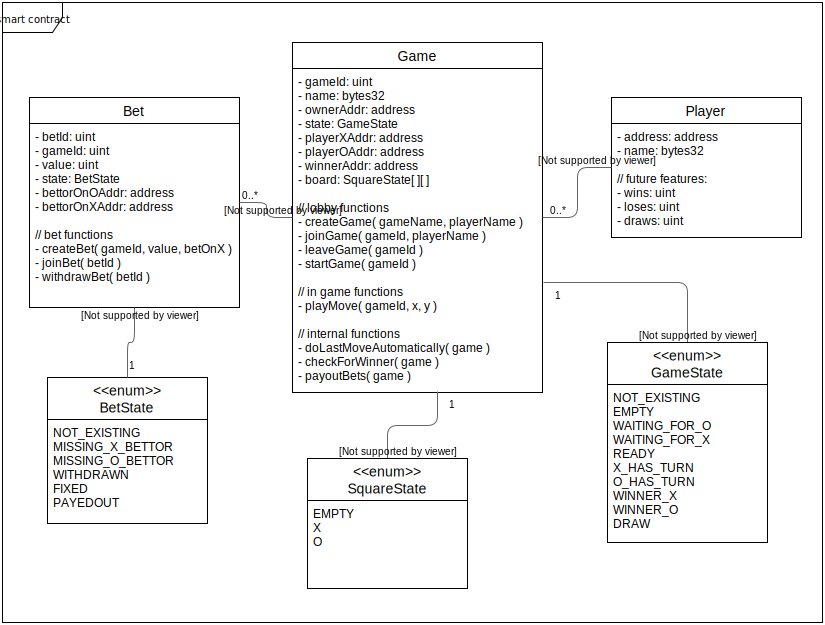
\includegraphics[scale=0.22]{res/sc_uml}
		\end{center}
		\caption{Class-Diagram of the \ac{sc}}
		\label{fig:sc_uml}
	\end{figure}
\section{Game Walk-through}
%logic and modell
